\chapter{Background}

The motivation behind solving chess puzzles, especially under time pressure, is
to improve one's pattern recognition abilities. It has been shown
\cite{thoughtAndChoice} that chess players do not have a square-by-square
recollection of the chess board during play. Instead, they rely on
interactions, and potential interactions of pieces in a more abstract sense.
This is made strikingly clear by a chess player's drawing of a position from
memory. (Figure \ref{deGrootFigure})

De Groot writes, `the pieces themselves do not appear in the drawing: rather
the lines of force that go out from them'. This heuristic allows expert human
players to quickly hone in on the correct moves,\cite{bilalic2010mechanisms}
and significantly reduces their search space, when compared to a naive
brute-force search, which is the most common strategy for chess engines. When
analysing positions, even the most basic chess engines are able to calculate
the most accurate line (except some pathological cases), but they are unable to
draw similarities between different positions.

\begin{figure}[H]
    \centering
    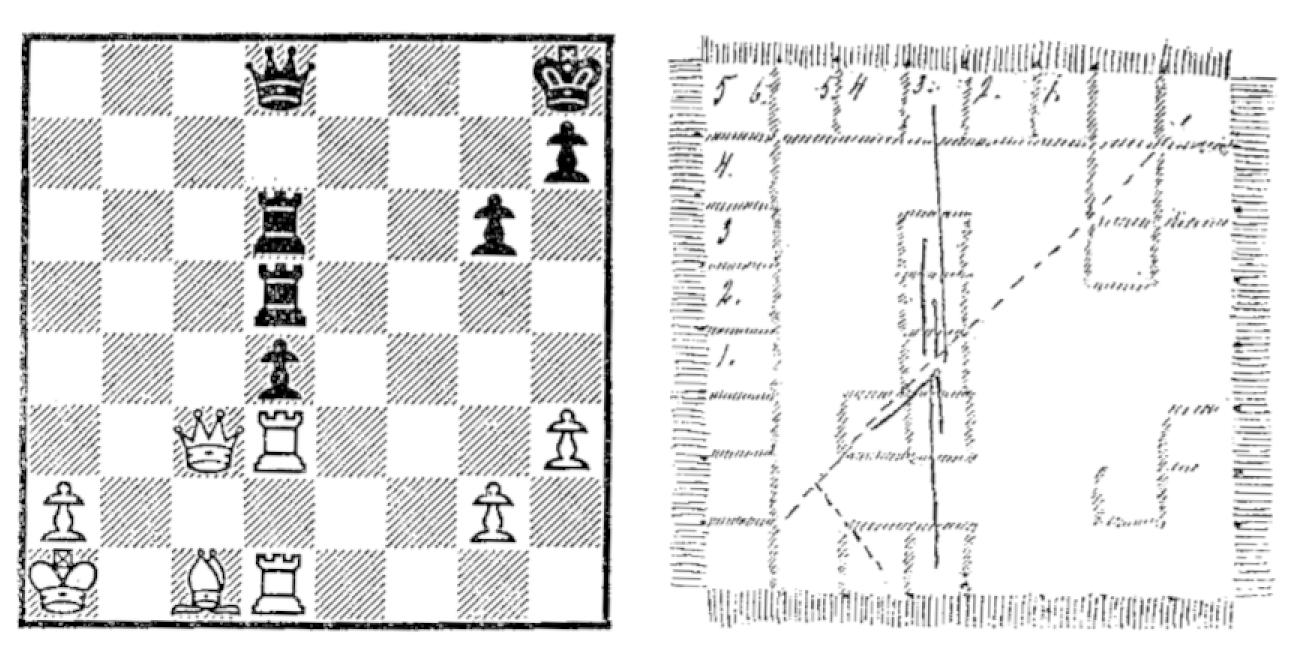
\includegraphics[width=0.9\linewidth]{background/img/deGroot.png}
    \caption{Taken from de Groot's `Thought And Choice In Chess'.\cite{thoughtAndChoice}}
    \label{deGrootFigure}
\end{figure}

In Figures \ref{chess1}, \ref{chess2}, 2 chess positions are shown, featuring
\emph{back-rank checkmates} -- one of the first tactical patterns that a
beginner might learn. A castled king is forced to stay on the back-rank due to
the configuration of his men, and an opposing heavy piece exploits this
weakness by delivering checkmate. It is already non-trivial to programmatically
identify this type of tactic, as a checkmate delivered to a king on the back
rank is not necessarily a \emph{back-rank checkmate}.

Given positions similar to ones like these, how does one draw similarities
between the abstract relations of the heavy piece, king, and vulnerable back
rank?

\begin{figure}[H]
    \begin{minipage}{0.475\textwidth}
        \centering
        \chessboard[setfen=6k1/5ppp/8/8/8/8/r4PPP/1R4K1 w - - 0 1]
        \caption{A trivial back-rank checkmate, white mates with \texttt{Rb8\#}.}
        \label{chess1}
    \end{minipage}
    \hspace{0.05\textwidth}
    \begin{minipage}{0.475\textwidth}
        \centering
        \chessboard[setfen=6k1/5ppp/1p1Q4/p3p1B1/Pn4P1/1q6/1Pr4P/K6R w - - 1 2]
        \caption{White mates with \texttt{Qd8\#}.}
        \label{chess2}
    \end{minipage}
\end{figure}

\section{Chess Notation}

For many decades, the standard for chess notation has been the Algebraic
System, where, generally speaking, moves are encoded by the piece abbreviation
(\texttt{Q} for queen, \texttt{K} for king, \texttt{N} for kNight) and a
reference to the destination square, which can be any letter \texttt{a-h} and
any number \texttt{1-8}.\cite{fideNotation} We assume that the reader is
familiarwith the basic chess rules.

When storing chess games and positions in a computer-readable format was
required, many formats were proposed by various people, but Portable Game
Notation (PGN) and Forsyth-Edwards Notation (FEN) stuck.\cite{pgnNotation}

\subsection{Portable Game Notation (PGN)}

PGN is a specific way to write chess moves in a text file. An example, taken
from Section 2.3 of the PGN Standard \cite{pgnNotation} is shown below. Along
with some metadata at the top of the file (player names, location, etc.\@), the
chess moves are written in algebraic notation, with an incrementing move
counter. In this example, Fischer played \texttt{e4} as his first move, with
Spassky responding with \texttt{e5}. The game ended in a draw on Spassky's 43rd
move.

\begin{verbatim}
[Event "F/S Return Match"]
[Site "Belgrade, Serbia JUG"]
[Date "1992.11.04"]
[Round "29"]
[White "Fischer, Robert J."]
[Black "Spassky, Boris V."]
[Result "1/2-1/2"]

1. e4 e5 2. Nf3 Nc6 3. Bb5 a6 4. Ba4 Nf6 5. O-O Be7 6. Re1 b5 7. Bb3 d6 8. c3
O-O 9. h3 Nb8 10. d4 Nbd7 11. c4 c6 12. cxb5 axb5 13. Nc3 Bb7 14. Bg5 b4 15.
Nb1 h6 16. Bh4 c5 17. dxe5 Nxe4 18. Bxe7 Qxe7 19. exd6 Qf6 20. Nbd2 Nxd6 21.
Nc4 Nxc4 22. Bxc4 Nb6 23. Ne5 Rae8 24. Bxf7+ Rxf7 25. Nxf7 Rxe1+ 26. Qxe1 Kxf7
27. Qe3 Qg5 28. Qxg5 hxg5 29. b3 Ke6 30. a3 Kd6 31. axb4 cxb4 32. Ra5 Nd5 33.
f3 Bc8 34. Kf2 Bf5 35. Ra7 g6 36. Ra6+ Kc5 37. Ke1 Nf4 38. g3 Nxh3 39. Kd2 Kb5
40. Rd6 Kc5 41. Ra6 Nf2 42. g4 Bd3 43. Re6 1/2-1/2 
\end{verbatim}

The main advantages of PGN are the ease with which it can be read by a human
\cite{pgnNotation} and, given its consistent structure, the simplicity of
parsing it programmatically. This led PGN to become widely adopted and
recognised by almost all chess software. However, a downside of PGN is that it
is difficult to retrieve a position at a given move -- it must be recalculated
by tracing the moves of the game from the start.

\subsection{Forsyth-Edwards Notation (FEN)}

An alternative notation used for static chess positions is FEN. This is much
more compact than PGN, as no metadata about the game is stored other than the
state of the board. Below is an example FEN string for the board in Figure
\ref{chessKGA}.

\begin{verbatim}
rnbqkbnr/pppp1ppp/8/8/4Pp2/5N2/PPPP2PP/RNBQKB1R b KQkq - 1 3
\end{verbatim}

\begin{figure}[H]
    \centering
    \chessboard[setfen=rnbqkbnr/pppp1ppp/8/8/4Pp2/5N2/PPPP2PP/RNBQKB1R b KQkq - 1 3]
    \caption{King's Gambit Accepted}
    \label{chessKGA}
\end{figure}

In FEN, pieces have their standard one-letter names, but pawns are explicitly
referred to with \texttt{P} or \texttt{p}. The number of consecutive empty
squares is denoted by an integer between \texttt{1} and \texttt{8}. The case of
the letter dictates what colour the chessman is: uppercase for white, and
lowercase for black. The arrangement of pieces is stored per rank,
left-to-right, with the first appearing rank in the string corresponding to
rank 8 on the board, and forward slashes delimiting the ranks. In the given
example, the 6th rank is stored as \texttt{8}, meaning there are 8 consecutive
empty squares on this rank. The 4th rank is stored as \texttt{4Pp2}, meaning
there are 4 empty squares, followed by a white pawn, then a black pawn, then 2
more empty squares.

The remaining characters store other information about the board. The single
\texttt{b} means it is Black to move; the string \texttt{KQkq} means White can
castle kingside (\texttt{K}) and queenside (\texttt{Q}), and Black can castle
both ways too (\texttt{kq}). If castling was not possible, this would be
denoted as \texttt{-}. The final 3 characters are en passant\footnote{French
for `in passing'. A special move where a pawn that advanced two squares can
be captured by an enemy pawn as if it was on the square behind. This is an
unending source of confusion for beginner players.} file, number of halfmoves
since the last pawn move or capture\footnote{Used for the fifty move draw
rule.}, and the number of full moves played.

\subsection{Bitboards}

When implementing chess programs on a computer, neither PGN or FEN are applicable
as they are difficult and slow to analyse. Instead, there are a number of various
numerical approaches to storing a chess position, with bitboards being one of the
bigger ones. One of the first mentions of Bitboards was in 
Adel'son-Vel'skii et al.\@'s 1970 paper.\cite{bitboardsRussian} 

Described informally, a bitboard is a collection of 12 64-bit integers, where
each integer corresponds to a piece type and colour. The bits of that integer
encode the position of a piece on the board: a piece on h1 activates the 1st
(least-significant) bit. Since modern processors utilise 64 bits, this makes
bitboards very fast -- especially when using other bitmaps to check for 
piece attack maps and piece interactions. In fact, bitboards are used by
Stockfish,\cite{stockfishBitboard} one of the strongest chess engines today.

\section{Examples of Chess Puzzle Themes}

In this section, we list a collection of common chess tactics which occur in
puzzles, and on a wider scale, games. Some of the positions are taken from the
chess.\@com blog.\cite{chesscomTactics}

\begin{figure}[H]
    \begin{minipage}{0.475\textwidth}
        \centering
        \chessboard[setfen=5r1k/4q1pp/3n2B1/1R5Q/8/7P/6P1/7K w - - 0 1]
    \end{minipage}
    \hspace{0.05\textwidth}
    \begin{minipage}{0.475\textwidth}
        \textbf{Mate In One}
        
        White wins in one move with \texttt{1.Qxh7\#}. There are many variants
        of simple checkmates, some of which are covered below.

    \end{minipage}
\end{figure}

\begin{figure}[H]
    \begin{minipage}{0.475\textwidth}
        \centering
        \chessboard[setfen=6k1/5ppp/3r4/8/8/3q4/5PPP/R2B2K1 b - - 0 1]
    \end{minipage}
    \hspace{0.05\textwidth}
    \begin{minipage}{0.475\textwidth}
        \textbf{Back-Rank Mate}
        
        Black wins with \texttt{1...Qxd1+ 2.Rxd1 Rxd1\#}. These positions occur
        very often when a king is castled, and the pawns surrounding the king
        on the 2nd/7th rank are preventing his escape to a different rank. A
        heavy piece\footnote{Rook or queen.} delivers the checkmate
        single-handedly.

    \end{minipage}
\end{figure}

\begin{figure}[H]
    \begin{minipage}{0.475\textwidth}
        \centering
        \chessboard[setfen=q2r3k/6pp/8/3Q2N1/8/8/5PPP/6K1 w - - 0 1]
    \end{minipage}
    \hspace{0.05\textwidth}
    \begin{minipage}{0.475\textwidth}
        \textbf{Smothered Mate}
        
        After \texttt{1.Nf7+ Kg8}, White delivers a \emph{double check} with
        \texttt{2.Nh6+}. Since Black is unable to remove both attacks on his
        king in one move, he is forced to move his king. \texttt{2...Kf8} leads
        to immediate mate with \texttt{3.Qf7\#}, so Black runs to the corner
        with \texttt{2...Kh8}. The white queen is sacrificed with
        \texttt{3.Qg8+ Rxg8}, entombing the black king in the corner. The white
        knight delivers checkmate with \texttt{4.Nf7\#}.

    \end{minipage}
\end{figure}

\begin{figure}[H]
    \begin{minipage}{0.475\textwidth}
        \centering
        \chessboard[setfen=r2qk1nr/ppp2ppp/2np4/4p3/1b2P1b1/2NPBN2/PPP2PPP/R2QKB1R w KQkq - 2 6]
    \end{minipage}
    \hspace{0.05\textwidth}
    \begin{minipage}{0.475\textwidth}
        \textbf{Absolute and Relative Pins}
        
        In this position, Black's bishops are pinning White's knights on
        \texttt{c3} and \texttt{f3}. The white knight on \texttt{c3} is under
        an \emph{absolute pin} from the black bishop on \texttt{b4}, as moving
        it is illegal. The white knight on \texttt{f3} is under a
        \emph{relative pin} from the other black bishop on \texttt{g4}. Whilst
        moving this knight is legal, it is rarely done, as the bishop is then
        able to capture the white queen on \texttt{d1}.

    \end{minipage}
\end{figure}

\begin{figure}[H]
    \begin{minipage}{0.475\textwidth}
        \centering
        \chessboard[setfen=2r3k1/8/8/n1n2N2/8/8/1P6/6K1 w - - 0 1]
    \end{minipage}
    \hspace{0.05\textwidth}
    \begin{minipage}{0.475\textwidth}
        \textbf{Fork}
        
        Forks come in multiple flavours, as multiple pieces are able to fork.
        Perhaps the most common is the knight fork, an example of which is
        possible on the board with \texttt{1.Ne7+}. The knight is attacking
        both the black rook on \texttt{c8} and black king on \texttt{g8}, and
        black is unable to capture the knight. After moving the king, black
        gives up the rook for a knight -- an unfavourable exchange.\\~\\The
        double pawn advance \text{1.b4} is also a fork. Black's knights are
        attacked and whilst they are able to defend each other, Black cannot
        move both to safety. One of them will be captured by the pawn.

    \end{minipage}
\end{figure}

\begin{figure}[H]
    \begin{minipage}{0.475\textwidth}
        \centering
        \chessboard[setfen=r2qkbnr/ppp2ppp/2np4/4N3/2B1P3/2N4P/PPPP1PP1/R1BbK2R w KQkq - 0 7]
    \end{minipage}
    \hspace{0.05\textwidth}
    \begin{minipage}{0.475\textwidth}
        \textbf{Attack On \texttt{f2}/\texttt{f7}}

        The \texttt{f2} and \texttt{f7} squares are very vulnerable for White
        and Black, respectively. At the beginning of the game, these squares
        are defended only by the king. If neglected, a quick attack, or even a
        sacrifice, can be devastating.\\~\\In this position, after sacrificing
        the queen, White's bishop can capture the weak pawn on \texttt{f7},
        leading to \texttt{1.Bxf7+ Ke7 2.Nd5\#}. 
        

    \end{minipage}
\end{figure}


\section{Related Work}

\subsection{A Language For Encoding Piece Relationships}

In `A description language for chess',\cite{chessLanguage} L\'{o}pez-Michelone
et al.\@ describe a language to search across chess positions. The main
features of this language are descriptions for a chess piece
attacking/defending another, attacking/defending a square, being located at a
square, a square not being available for the enemy king, and the structure of
white/black pawns on the board.

With their novel language, they are able to search a chess database for a
pre-determined pattern, such as the \emph{Greek gift sacrifice}, defined in the
language as `\texttt{kg8, pf7, pg7, B(ph7), Nf3, Qd1, Pe5}. With inspiration
from the FEN notation, this string corresponds to a black king on g8
(\texttt{kg8}), black pawns on f7, g7; a white bishop attacking a black pawn on
h7 (\texttt{B(ph7)}), a white knight on f3 (ready to deliver a check with
\texttt{Ng5+}, a common motif in \emph{Greek gift sacrifices}), a white queen
on d1 (\texttt{Qd1}), and finally, a white pawn on e5 (\texttt{Pe5}),
dislodging the usual black knight on f6.

This returns positions such as the one shown in Figure \ref{chess3}. After
\texttt{16...Be7 17. O-O}, Black blundered with \texttt{17...Bxa3??}, after
which, a \emph{Greek gift sacrifice} (\texttt{18.Bxh7!}, shown in Figure
\ref{chess4}) was made, eventually leading to a win for White.

\begin{figure}[H]
    \begin{minipage}{0.475\textwidth}
        \centering
        \chessboard[setfen=r1b2rk1/qp3ppp/p1n1pb2/4P3/3P4/P1BB1N2/5PPP/1R1QK2R b K - 0 16]
        \caption{\textbf{Pirc, V -- Porreca, G}, YUG-ITA m 1953, move 16.}
        \label{chess3}
    \end{minipage}
    \hspace{0.05\textwidth}
    \begin{minipage}{0.475\textwidth}
        \centering
        \chessboard[setfen=r1b2rk1/qp3ppB/p1n1p3/4P3/3P4/b1B2N2/5PPP/1R1Q1RK1 b - - 0 18]
        \caption{\textbf{Pirc, V -- Porreca, G}, YUG-ITA m 1953, move 18. Black resigned after 6 moves.}
        \label{chess4}
    \end{minipage}
\end{figure}

Their language is also able to deal with some light variations, as it is able
to identify the games shown in Figures \ref{chess5}, \ref{chess6}. In both of
these positions, White has the brilliant move \texttt{1.Qh6+!!}, following
with \texttt{2.Rh8\#} if \texttt{1...Kxh6}, and either \texttt{2.Rf7\#} or
\texttt{2.Rb7+} (leading to a quick mate) if \texttt{1...gxh6}. 

This pattern, whilst very rare, is undeniably identical between the 2 games.
The unavailability of the \texttt{g6} square to the enemy king, combined with
the harmony of White's pieces leads to the same tactic in both games.

\begin{figure}[H]
    \begin{minipage}{0.475\textwidth}
        \centering
        \chessboard[setfen=2R5/4bppk/1p1p4/5R1P/4PQ2/5P2/r4q1P/7K w - - 5 50]
        \caption{\textbf{Carlsen, M -- Karjakin S}, World Chess Championship 2016, move 50.}
        \label{chess5}
    \end{minipage}
    \hspace{0.05\textwidth}
    \begin{minipage}{0.475\textwidth}
        \centering
        \chessboard[setfen=5R2/bp4pk/2n3p1/P7/P1q3bP/6P1/3Q3K/1R6 w - - 1 32]
        \caption{\textbf{Popov, N -- Novopashin, A}, URS-ch otbor 1979, move 32.}
        \label{chess6}
    \end{minipage}
\end{figure}

The work of L\'{o}pez-Michelone et al.\@ is a promising proof of concept that
shows the power of a language that allows to specify piece relationships on a
more abstract level than previously possible. The biggest drawback of their
solution, as mentioned by the authors, is the fact that this language still
requires an expert with pre-existing extensive knowledge to encode the tactics
into their language. The authors hypothesise that automatic recognition of
these patterns is likely some sort of neural network, which is one of the many
possible directions of this project.

\subsection{CQL: Chess Query Language}

The Chess Query Language (CQL), as invented by Costeff,\cite{cql} is another
implementation of an advanced way to find chess positions in a given database.
Since its inception in 2004, it has grown and is able to support very powerful,
sometimes esoteric, queries to find predefined patterns.

An example of such a query is provided on the CQL website,\cite{cqlSmothered}
and is shown in Figure \ref{cql} for reference. In this query, \texttt{btm}
means `black-to-move` and \texttt{mate} means checkmate is played. This
language is incredibly powerful and terse, as it allows specifying complicated
piece relationships and supports quality-of-life features such as matching
mirror positions or reversed-colour positions.

\begin{figure}[H]
    \centering
    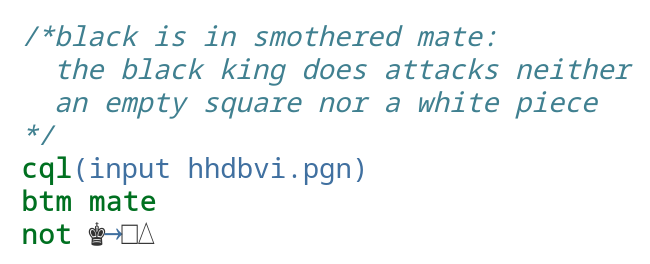
\includegraphics[width=0.45\linewidth]{background/img/cql.png}
    \caption{A CQL query to find positions where smothered mate occured.}
    \label{cql}
\end{figure}

In addition to the Costeff's CQL, there is a from-scratch clone of CQL6
which includes extra features and supports other chess
variants.\cite{cqli}

\subsection{lichess.org Puzzle Database}

\url{https://lichess.org} is a popular, open-source chess website which often
publishes the games that have been played by players of all skill levels on it.
As part of this, Lichess has published over 3.6 million rated and tagged puzzle
positions.\cite{lichessPuzzles} To generate these, 300 million games were
analysed with a powerful chess engine to find critical positions in which a
move must be played to capitalise on the opponent's mistake. These puzzles were
initially tagged to 124 manually created themes,\cite{lichessXML} which were
identified by a python implementation.\cite{lichessTagger} 

As various users of the site solved the puzzles, and manually highlighted the
themes that they felt occured in the puzzle, the ratings and tags of the puzzle
database evolved until their current state.

This database is invaluable for this project, and can likely serve either as
input, or as a baseline to compare the results to.

\subsection{Recognition of the \emph{Greek Gift Sacrifice} In Chess Games}

Kub\'{a}t et al.\@ report their findings on a program \cite{middlegamePatterns}
to identify the \emph{Greek gift sacrifice} in chess middlegames.\footnote{The
phase of the chess game where most pieces are developed and the kings are
positioned away from danger.} They found success, partly thanks to their
detailed representation of the board, where each square is represented by 71
binary attribites \cite{middlegamePatterns} to encode the piece on the square
and the possible squares which are reachable by this piece. 

These attributes were also supplemented by 59 other binary attribites which
were devised by expert chess players, and represent the more complex, but still
quantifiable relationships.\cite{middlegamePatterns} These include open files,
control of vulnerable squares, piece activity, and so on.

Kub\'{a}t et al.\@ achieved an 87.7\% classification performance on detecting
whether a position features a successful \emph{Greek gift sacrifice} on
relatively small (<200 positions) datasets. This work is promising, but more
investigation is needed given their analysis of only one pattern with a
decision tree algorithm. Also, their program still relied on predetermined
chess patterns, which introduces bias and might miss intricate similarities
between positions.

\subsection{A Novel Chess Board Representation For Convolutional Neural Networks}

In Sabatelli's thesis,\cite{chessCNN} the effectiveness of neural networks to
analyse whether a chess position is winning or losing is explored, without
creating specific look-ahead algorithms. This is a very challenging task, but
as part of the analysis, the author proposed manually encoded features to a
convolutional neural network (CNN) to help identify strong patterns within the
position. 

Some of these include an extra feature if the opponent is in check, specifying
the squares controlled by a piece exerting a pin on a different piece, centre
control, and vulnerable squares.\cite{chessCNN} These are well known
heuristics that are often taught to beginner-intermediate chess players, and
the author claims that these additional layers are `extremely representative
of the chess positions', and cause the CNN to outperform a naive,
fully-connected neural network.

This work is also a promising result, as it shows that these chess patterns,
albeit manually quantified, are valuable for an algorithm when analysing a
given chess position.

\subsection{Chess Moves As Kernels For Texture Classification}

In this study, Tuncer et al.\@ propose novel kernels for efficient feature
extraction in the task of texture detection.\cite{chessKernel} These 5x5
kernels are directly based on the move a rook, bishop, knight, and their
combinations. 

Whilst not directly applicable to the context of chess puzzle analysis, this
work shows that it may be possible to include these kernels in an CNN-based
analysis of the chess position. It would be interesting to apply to the other
CNN chess work (e.g. Sabatelli's thesis,\cite{chessCNN} discussed above) and
analyse its effect on the success of the technique.

\subsection{A Computational Model for Estimating the Difficulty of Chess
Problems} \label{chessTreesOverview}

Stoiljkovikj et al.\@ explore estimation of difficulty of chess problems in
this paper.\cite{chessTrees} By using a powerful chess engine, they generate a
tentative move tree of forcing or winning moves in a given position, mirroring
the process of calculating a variation for a chess player. 

By creating higher level metrics based off these trees (e.g. branching factor,
piece variety, move distances) and applying standard statistical machinery, the
authors are able to categorise the puzzles into various difficulty levels with
some success.

Their unique `meaningful search tree'\cite{chessTrees} approach to analysing
chess puzzle moves is novel, and we believe it has more potential for this
problem. Specifically, adding more chess-related metadata to the tree nodes (is
the move a fork, skewer, etc.?\@) could improve the performance and allow
better classification, and would be interesting to perform.

\subsection{Chess2vec: Learning Vector Representations for Chess}

In this paper, Kapicioglu et al.\@ investigate and report on their results in
finding $d$-dimensional vector representations of the standard way to represent
a chess board in machine learning -- a bitboard,\cite{chess2vec} which is
equivalent to a $8\times8\times12$ binary tensor. 

With this naive approach, the authors make the observation that each chess
square is a 12-dimensional vector, which is independent of the board. By adding
a board hash, they segregate the pieces, making their vector representations
depend on the board state. With this method, the authors claim to predict
$8.8\%$ of Stockfish moves correctly,\cite{chess2vec} which is an impressive
statistic given no chess logic or ruleset was explicitly implemented.

This is a promising result that suggests that vector representations of pieces
on a chess board can have unexpected performance, and it would be interesting
to build upon the authors' work.

\subsection{The Chess Transformer: Mastering Play using Generative Language Models}

Noever et al.\@ demonstrate the ability of transformers to learn the rules of
chess and complex gameplay by analysing PGN games with a fine-tuned GPT-2
transformer.\cite{chessTransformer} By treating PGN games as a sequence of
natural language words, the authors show successful results and are able to
generate new games without specifying chess rules.

A key downside of their work is that their model generates illegal moves, which
have to be filtered manually using a chess library.\cite{chessTransformer} This
`hallucination' effect is a downside of using transformers, and other
generative techniques, in the topic of chess. 

\subsection{Automatic Recognition of Similar Chess Motifs} \label{chessMotifsOverview}

In their thesis,\cite{chessMotifs} Bizjak et al.\@ develop a method to retrieve
similar chess positions among a variety of tactically sharp examples. Building
upon the naive `static' similarity (piece locations, pawn structure, etc.\@),
they implement various `dynamic' similarity metrics (whether captures occur,
attacks happen, sacrifices happen, etc.\@ in the optimal move chain). It is
well known \cite{thoughtAndChoice}\cite{bilalic2010mechanisms} that chess
players often think about positions in this dynamic way. This is further
reinforced by an example given in the thesis, where a small static perturbation
causes previously dynamically similar positions to have nothing in
common.\cite{chessMotifs}

This work is incredibly close to the goal of our project, and it has plenty of
interesting approaches and ideas. Importantly, their results are successful:
when a chess expert was asked to identify similar positions, they chose the
same ones that Bizjak et al.\@'s program did.\cite{chessMotifs} Whilst this is
not a faultless evaluation metric, it shows that there is potential within
their approach.


\section{Ethical discussion}

This project has few, if any, ethical considerations that need to be made. The
biggest concern is the source of the large datasets that may be used in this
project, namely, the Lichess puzzle database.\cite{lichessPuzzles} However,
this database, along with all Lichess games is released under the Creative
Commons CC0 license -- meaning there is no restriction in its use.

Each puzzle in this database contains a link to the game from which it was
extracted, and this contains a Lichess username, which is deanonymising. In the
initial data processing stage, these links are going to be removed, as they are
unnecessary for the goals of the project.

Another concern is the use of, and reference to specific chess games and the
players in them, and various chess compositions\footnote{An artificially
created position to showcase a uniquely challenging, rare, or otherwise
interesting theme.} with their authors. Other than proper reference to the
creators of the game or composition, there are no other considerations to be
made.

